% !TEX program = xelatex
% !BIB program = bibtex
% Connect6 Game Engine (tbe) — report, Russian draft.
% Compile with XeLaTeX:  xelatex report && bibtex report && xelatex report && xelatex report
\documentclass[a4paper,10pt,twocolumn]{article}

\usepackage[margin=1.8cm,columnsep=0.7cm]{geometry}
\usepackage{fontspec}
\usepackage{polyglossia}
\setmainlanguage{russian}
\setotherlanguage{english}
\gappto\captionsrussian{\renewcommand{\abstractname}{Abstract}\renewcommand{\refname}{References}}
% First available font with Cyrillic: PT Serif (macOS, Overleaf) -> Times New Roman -> FreeSerif -> DejaVu Serif
\IfFontExistsTF{PT Serif}{\setmainfont{PT Serif}}{%
  \IfFontExistsTF{Times New Roman}{\setmainfont{Times New Roman}}{%
    \IfFontExistsTF{FreeSerif}{\setmainfont{FreeSerif}}{\setmainfont{DejaVu Serif}}}}
\IfFontExistsTF{PT Sans}{\setsansfont{PT Sans}}{\IfFontExistsTF{FreeSans}{\setsansfont{FreeSans}}{\setsansfont{DejaVu Sans}}}
\IfFontExistsTF{PT Mono}{\setmonofont[Scale=0.9]{PT Mono}}{\setmonofont[Scale=0.85]{DejaVu Sans Mono}}

\usepackage{amsmath,amssymb}
\usepackage{graphicx}
\usepackage{booktabs,tabularx,multirow}
\usepackage[table]{xcolor}
\usepackage{caption,subcaption}
\usepackage{enumitem}
\newenvironment{points}{\begin{enumerate}[label=(\arabic*),leftmargin=*,itemsep=2pt,topsep=3pt]}{\end{enumerate}}
\usepackage{tikz}
\usetikzlibrary{positioning,arrows.meta,calc,fit,backgrounds,shapes.misc}
\usepackage{pgfplots}
\pgfplotsset{compat=1.17}
\usepackage[round,authoryear]{natbib}
\setcitestyle{aysep={,},citesep={;}}
\usepackage{titlesec}
\usepackage[colorlinks=true,citecolor=blue!55!black,linkcolor=black,urlcolor=blue!55!black]{hyperref}
\usepackage{url}

\captionsetup{font=small,labelfont=bf,skip=4pt}
\titleformat*{\section}{\large\bfseries}
\titleformat*{\subsection}{\normalsize\bfseries}
\setlength{\parskip}{0.2em}
\newcommand{\todo}[1]{\textcolor{red}{[#1]}}
\newcommand{\code}[1]{\texttt{#1}}
\definecolor{cblue}{HTML}{2A78D6}
\definecolor{corange}{HTML}{EB6834}
\definecolor{cgreen}{HTML}{1BAF7A}
\definecolor{board}{HTML}{E2C27A}
\renewcommand{\arraystretch}{1.12}

% ---------- board drawing helpers (column c, row r; row A at the top, as in the GUI)
\tikzset{
  bstone/.style={circle,fill=black,inner sep=0pt,minimum size=3.4mm},
  wstone/.style={circle,fill=white,draw=black,line width=0.4pt,inner sep=0pt,minimum size=3.4mm},
  xmark/.style={cross out,draw=red,line width=1pt,inner sep=0pt,minimum size=2.4mm},
}
% \board{c0}{c1}{r0}{r1}: grid from column c0 to c1, rows r0 to r1, with letters
\newcommand{\board}[4]{%
  \fill[board] (#1-0.6,-#3+0.6) rectangle (#2+0.6,-#4-0.6);
  \foreach \c in {#1,...,#2} {\draw[black!60,line width=0.3pt] (\c,-#3) -- (\c,-#4);
     \node[font=\tiny\ttfamily,above] at (\c,-#3+0.45) {\pgfmathparse{int(\c+64)}\char\pgfmathresult};}
  \foreach \r in {#3,...,#4} {\draw[black!60,line width=0.3pt] (#1,-\r) -- (#2,-\r);
     \node[font=\tiny\ttfamily,left] at (#1-0.45,-\r) {\pgfmathparse{int(\r+64)}\char\pgfmathresult};}
}
\newcommand{\B}[2]{\node[bstone] at (#1,-#2) {};}
\newcommand{\W}[2]{\node[wstone] at (#1,-#2) {};}

\title{\textbf{Connect6 Game Engine}\\[0.3em]\large engine: \texttt{tbe}}
\author{Tamara Besedina}
\date{November 2026}

\begin{document}
\maketitle
\begin{abstract}
\noindent
Цель работы --- движок для игры Connect6, совместимый с интерфейсом Connect6GUI/\allowbreak{}Connect6Engine \citep{connect6gui}, который отвечает в реальном времени и использует веса оценочной функции, в том числе обученные методом машинного обучения \citep{statement}. Движок \code{tbe} развивался в пять версий: v1 --- минимакс на глубину два полных хода; v2 --- alpha-beta с упорядочиванием ходов и проверкой немедленных выигрышей и защит; v3 --- оценочная функция с угрозами по Wu--Huang и связностью по Liu; v4 --- quiescence search и forward pruning (основное ускорение, в 2.7 раза, v4 даёт forward pruning, а quiescence в основном добавляет стоимость); v5 --- обучение весов бутстрэппингом от поиска, которое в итоге показало, что исходные веса лучше, так что фактически v5 = v4. Обучение воспроизводимо сходится из разных стартов, но не даёт выигрыша в силе игры (45.8\,\% очков против ручных весов). Итоговая версия проходит все 12 тестовых позиций (выигрыш и защита за 1--3 хода) против Cloudict, в стартовых позициях держится против него в среднем 11 своих ходов (v1 --- 6.5) и занимает второе место в турнире после Cloudict.
\end{abstract}

% =====================================================================
\section{Introduction}

Connect6 --- игра двух игроков из семейства $k$-in-a-row \citep{wu2005family}. Чёрные первым ходом ставят один камень, далее игроки по очереди ставят по \emph{два} камня на свободные пересечения доски $19\times19$; побеждает тот, кто первым построит ряд из шести и более камней по горизонтали, вертикали или диагонали. Правило 1--2--2 делает игру сбалансированной: после своего хода у каждого игрока на доске ровно на один камень больше, чем у соперника \citep{wu2005family}.

Для перебора игра очень сложна: на пустой доске ход выбирается из $\binom{361}{2}\approx 65\,000$ пар клеток, в середине партии --- из десятков тысяч. Поэтому даже глубина в два полных хода невозможна без сильного ограничения кандидатов, отсечений и хорошей оценки позиции.

\paragraph{Project structure.} Работа построена как цепочка версий от v1 до v5: каждая следующая добавляет улучшение. В v4 сразу добавлены две техники (quiescence и forward pruning); их вклад разделён отдельным экспериментом (раздел~\ref{sec:ablation}). Эксперименты выполнялись локально на MacBook Air (Apple M1, 8\,ГБ RAM, macOS 26.5.2): партии с человеком --- через ConnectMore GUI, тесты, турнир и обучение --- из терминала. Код: \todo{ссылка на GitHub}.

% =====================================================================
\section{State of the Art}\label{sec:sota}

\subsection{k-in-a-Row Games and Connect6}
Wu и Huang \citeyearpar{wu2005family} ввели семейство игр Connect($m,n,k,p,q$) и предложили Connect6 = Connect(19,19,6,2,1) как справедливую игру. Ключевое для нас понятие из их работы --- \emph{угроза}: позиция, в которой соперник должен потратить определённое число камней, чтобы не проиграть на следующем ходу. Если для защиты хватает одного камня --- это одиночная угроза, двух --- двойная; если двух не хватает, игрок с угрозой выигрывает. Поскольку за ход ставится два камня, мёртвая четвёрка (один конец закрыт) даёт одиночную угрозу, а открытая четвёрка --- двойную. Авторы также подчёркивают, что перекрывающиеся линии нельзя считать независимыми угрозами и что второй камень хода нужно выбирать уже после постановки первого.

\subsection{Game-Tree Search}
Базовый алгоритм --- минимакс с ограничением глубины и статической оценкой в листьях \citep{russell2020aima}. Alpha-beta даёт тот же результат, но отсекает ветви, которые не могут повлиять на решение; при идеальном порядке ходов число узлов уменьшается примерно до квадратного корня от минимакса \citep{knuth1975alphabeta}, поэтому упорядочивание ходов --- обязательная часть alpha-beta. При фиксированной глубине возникает \emph{эффект горизонта}: угроза сразу за границей поиска не видна. Quiescence search продолжает поиск в «нетихих» листьях только по тактическим ходам \citep{russell2020aima}. Forward pruning заранее отбрасывает ходы, которые эвристически выглядят слабыми, жертвуя точностью ради скорости. Предложенные в гайде таблицы транспозиций, history heuristic и дебютные книги \citep{statement} не реализованы.

\subsection{Connect6-Specific Methods}
Сильнейшие программы Connect6 опираются на поиск в пространстве угроз (threat-space search), предложенный Allis для гомоку \citep{allis1994}: рассматриваются только ходы, создающие угрозы, что позволяет находить форсированные выигрыши на большую глубину. Частный случай --- VCF (victory by continuous fours), последовательность ходов, каждый из которых создаёт угрозу; именно так Cloudict находит выигрыши. Wu и Lin \citeyearpar{wu2010rzop} строят на этой идее доказательный поиск по «зонам релевантности» --- областям доски, где обязана лежать защита. Liu \citeyearpar{liu_defensive} дополняет поиск угроз защитной стратегией и оценкой потенциальных линий: влияние камня убывает с расстоянием и не проходит через камень соперника; эту идею мы используем в признаке связности.

\subsection{Learning the Evaluation Function}
Оценку часто записывают как линейную комбинацию признаков (линии, угрозы) с весами. В программе NCTU6, многократном чемпионе компьютерных олимпиад по Connect6, веса сначала подбирались вручную по партиям с сильными игроками, а затем уточнялись TD(0)-обучением, что дало 57.95\,\% побед против исходной версии \citep{wu2012td}. Методичка предлагает генетический алгоритм \citep{statement}: популяция наборов весов, fitness --- результат партий между ними. Альтернатива --- обучение по позициям: TD-Leaf \citep{baxter2000tdleaf} подстраивает оценку под результат поиска из последующих позиций, бутстрэппинг от дерева поиска \citep{veness2009bootstrapping} --- под значение поиска в той же позиции, а Texel tuning \citep{texel} минимизирует логистическую ошибку между оценкой и меткой позиции.

Генетический алгоритм не был реализован, потому что fitness в GA --- результат партий: на одну оценку одного набора весов нужны десятки партий, на поколение --- сотни. Бутстрэппинг даёт метку для \emph{каждой} позиции, а не одну на партию, и дифференцируемую ошибку, поэтому за 15~минут самоигры получается несколько тысяч обучающих примеров и градиентная оптимизация.

\subsection{Reference Opponent: Cloudict}
Cloudict \citep{cloudict} --- открытый движок Connect6 на C++: alpha-beta на заданную глубину (у нас 2) с поиском VCF. Он служит эталонным соперником во всех тестах.

% =====================================================================
\section{Development}\label{sec:dev}

\subsection{Architecture}
Все версии имеют одну структуру из пяти модулей, заданную шаблоном преподавателя (рис.~\ref{fig:arch}): \code{main.py} запускает движок, \code{game\_engine.py} разбирает команды протокола, \code{search\_engine.py} содержит генератор ходов, оценку и поиск, \code{defines.py} --- константы и веса, \code{tools.py} --- доску и проверку победы. Доска $19\times19$ хранится в массиве $21\times21$ с рамкой. Ответы протокола идут в stdout, метрики поиска (узлы, отсечения, глубина, время) --- в stderr: GUI их игнорирует, а скрипты экспериментов читают.

\begin{figure*}[t]
\centering
\resizebox{\textwidth}{!}{%
\begin{tikzpicture}[
  box/.style={draw,rounded corners=2pt,align=center,font=\small,minimum height=9mm,inner sep=4pt,fill=white},
  ext/.style={box,fill=black!6},
  arr/.style={-{Stealth[length=2mm]},thick},
  lab/.style={font=\scriptsize,align=center}]
\node[ext] (gui) {ConnectMore GUI\\ / \code{benchmark.py}, \code{train.py}};
\node[box,right=1.6cm of gui] (main) {\code{main.py}\\ запуск};
\node[box,right=0.9cm of main] (ge) {\code{game\_engine.py}\\ протокол, доска партии,\\ лимит времени};
\node[box,right=1.5cm of ge] (se) {\code{search\_engine.py}\\ генератор ходов $\cdot$ оценка\\ alpha-beta $\cdot$ quiescence $\cdot$ FP};
\node[box,below=0.8cm of ge] (tools) {\code{tools.py}\\ ходы, победа, печать};
\node[box,below=0.8cm of se] (def) {\code{defines.py}\\ константы, \code{EVAL\_WEIGHTS}};
\node[ext,right=0.9cm of def] (lw) {\code{learned\_weights.json}\\ (v5)};
\draw[arr] (gui.north east) to[bend left=12] node[lab,above] {stdin: \code{new}, \code{move},\\ \code{next}, \code{depth} \ldots} (ge.north west);
\draw[arr] (ge.south west) to[bend left=12] node[lab,below] {stdout: \code{move XXXX}\\ stderr: \code{metrics \{\ldots\}}} (gui.south east);
\draw[arr] (main) -- (ge);
\draw[arr] (ge) -- node[lab,above] {позиция,\\ бюджет} (se);
\draw[arr] (se) -- (tools);
\draw[arr] (ge) -- (tools);
\draw[arr] (def) -- (se);
\draw[arr] (lw) -- (def);
\end{tikzpicture}}
\caption{Архитектура движка tbe и поток команд между GUI (или скриптами экспериментов) и движком. Модули одинаковы во всех версиях; от версии к версии меняется в основном \code{search\_engine.py}.}
\label{fig:arch}
\end{figure*}

\subsection{Communication Protocol and Time Control}
Движок понимает все команды задания (табл.~\ref{tab:protocol}). Команда \code{depth N} по заданию означает не глубину, а лимит в $N$ секунд на ход. Время контролируется так: поиск идёт итеративно (сначала глубина 1, потом 2), при каждом узле проверяется таймер, и при исчерпании бюджета возвращается лучший ход последней \emph{полностью} завершённой глубины. Небольшая часть бюджета оставляется на вывод ответа.

\begin{table*}[t]
\centering
\caption{Команды протокола Connect6GUI/\allowbreak{}Connect6Engine \citep{connect6gui} и их реализация в tbe.}
\label{tab:protocol}
\begin{tabularx}{\textwidth}{@{}lX@{}}
\toprule
Команда & Действие \\
\midrule
\code{name} & ответ \code{name tbe} \\
\code{new black} / \code{new white} & новая партия; движок играет за указанный цвет \\
\code{new xxx}, \code{black XXXX}, \code{white XXXX} & сброс и восстановление произвольной позиции по ходам (буквы A--S) \\
\code{next} & рассчитать ход для стороны, чья очередь \\
\code{move XXXX} & поставить ход соперника и сразу ответить своим (\code{move JKJL}; ход одним камнем --- \code{move JJ}) \\
\code{depth N} & лимит времени $N$ секунд на ход (не глубина дерева) \\
\code{print}, \code{help}, \code{exit}/\code{quit} & печать доски, справка, завершение \\
\code{vcf}, \code{unvcf} & принимаются и игнорируются, как требует задание \\
\bottomrule
\end{tabularx}
\end{table*}

\subsection{v1: Minimax Baseline}
Первая версия выполняет требования первой сессии методички.
\emph{Конец партии}: после каждого хода проверяется, не образовал ли поставленный камень шесть подряд в одном из четырёх направлений; полная доска без победы --- ничья.
\emph{Генератор ходов}: кандидаты --- пустые клетки в радиусе 3 от любого камня; они ранжируются простой локальной оценкой, берутся 12 лучших клеток и из них до 24 пар (оценка пары --- сумма оценок клеток). Это сознательно узкий генератор: полный перебор пар даже на глубину один невозможен.
\emph{Оценка}: для каждого окна из шести клеток без камней соперника считается число своих камней; оценка --- сумма чёрных минус сумма белых, победа $\pm10^6$, ничья 0.
\emph{Поиск}: минимакс на глубину 2 полных хода (ход и ответ).

\subsection{v2: Alpha-Beta Pruning and Move Ordering}
\emph{Alpha-beta.} Метод построен прямо на минимаксе v1 с теми же терминальными условиями и границей глубины; на одинаковом дереве он возвращает тот же ход (проверено тестом), но отсекает ветви при $\alpha\ge\beta$.

\emph{Упорядочивание и форсированные ходы.} Alpha-beta эффективна, только если сильные ходы рассматриваются первыми \citep{knuth1975alphabeta}, поэтому генератор стал умнее. (1) Если есть немедленный выигрыш, предлагаются только выигрывающие пары. (2) Иначе ищутся все окна соперника с 4--5 камнями, и предлагаются только пары, перекрывающие \emph{все} его способы выиграть следующим ходом; такие клетки входят в кандидаты независимо от лимита 12. Если защиты двумя камнями нет, поиск продолжается по обычным ходам, чтобы честно оценить проигрыш. (3) В спокойной позиции пара оценивается совместным изменением всех затронутых окон: два камня одного хода могут усиливать одну линию, а сумма оценок отдельных клеток этого не видит.

\emph{Оценка с весами.} Число камней в окне заменено весом, растущим в 4 раза на каждый камень: 1, 4, 16, 64, 256 за окно с 1\ldots5 своими камнями (обоснование --- в разделе~\ref{sec:v3}). Рис.~\ref{fig:v2game} --- пример партии v2 против человека.

\begin{figure*}[t]
\centering
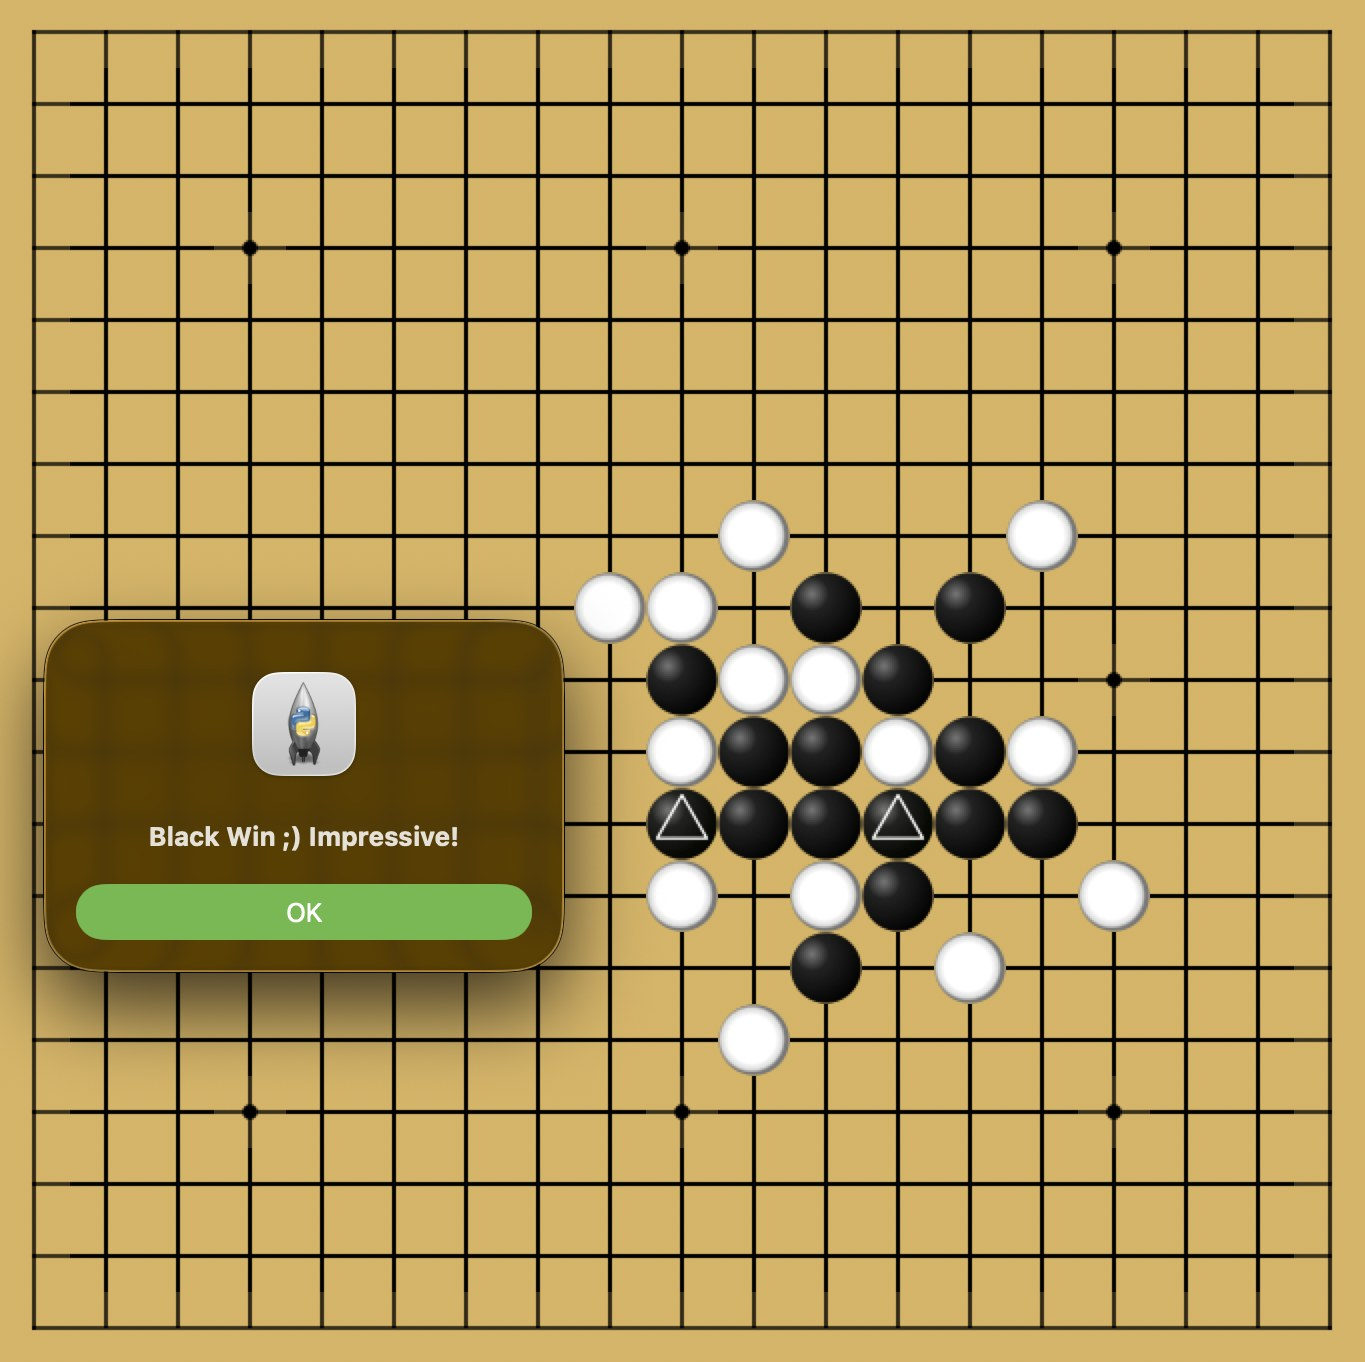
\includegraphics[width=0.48\textwidth]{figures/v2_vs_human.jpg}
\caption{Партия v2 (чёрные) против человека в ConnectMore GUI.}
\label{fig:v2game}
\end{figure*}

\subsection{v3: Threat-Based Evaluation}\label{sec:v3}
Третья версия реализует собственную оценочную функцию по литературе. Для каждого цвета считаются девять признаков (табл.~\ref{tab:features}, рис.~\ref{fig:features}):

\begin{itemize}\itemsep0pt
\item \code{line\_1}\ldots\code{line\_5} --- число окон из шести клеток, где у цвета 1\ldots5 камней, а камней соперника нет (окна, которые ещё могут стать шестёркой);
\item \code{threat\_1}, \code{threat\_2}, \code{threat\_3} --- угроза по Wu и Huang \citeyearpar{wu2005family}: для каждого окна с 4--5 камнями запоминаются пустые клетки, которыми его можно завершить, и ищется минимальное число камней, перекрывающих \emph{все} такие наборы (с учётом пересечений направлений). Флаг \code{threat\_1} --- хватает одного камня, \code{threat\_2} --- нужно два, \code{threat\_3} --- двух не хватает;
\item \code{connectivity} --- идея Liu \citeyearpar{liu_defensive}: по каждой линии, разделённой камнями соперника на участки длиной не меньше шести, каждая пара своих камней на расстоянии $d\le5$ даёт вклад $6-d$. Близкие камни ценнее, влияние не проходит сквозь камень соперника.
\end{itemize}

Оценка позиции --- взвешенная разность признаков:
\begin{equation}
E=\sum_{i} w_i\,\bigl(f_i^{\text{чёрные}}-f_i^{\text{белые}}\bigr),
\label{eq:eval}
\end{equation}
$E>0$ --- преимущество чёрных; победа $\pm10^6$ независимо от весов.

\begin{table*}[t]
\centering
\caption{Признаки оценочной функции v3 и ручные (экспертные) веса. Эти же веса используются в v4 и v5.}
\label{tab:features}
\begin{tabularx}{\textwidth}{@{}lrX@{}}
\toprule
Признак & Вес & Смысл \\
\midrule
\code{line\_1}\ldots\code{line\_5} & 1, 4, 16, 64, 256 & окна из 6 клеток с 1\ldots5 своими камнями без камней соперника; каждый камень $\times4$ \\
\code{threat\_1} & 600 & все немедленные выигрыши перекрываются одним камнем (мёртвая четвёрка) \\
\code{threat\_2} & 3000 & нужно два камня (открытая четвёрка) \\
\code{threat\_3} & 15000 & двух камней не хватает --- защиты нет \\
\code{connectivity} & 2 & сумма $(6-d)$ по парам своих камней на одной незаблокированной линии, $d\le5$ \\
\bottomrule
\end{tabularx}
\end{table*}

\begin{figure*}[t]
\centering
\begin{subfigure}[t]{0.36\textwidth}\centering
\begin{tikzpicture}[scale=0.42]
\board{1}{12}{1}{3}
\B{4}{2}\B{5}{2}\B{7}{2}\W{11}{2}
\draw[cblue,line width=1.2pt,rounded corners=2pt] (1.55,-1.62) rectangle (7.45,-2.38);
\draw[cgreen,line width=1.2pt,rounded corners=2pt,dashed] (2.55,-1.5) rectangle (8.45,-2.5);
\draw[corange,line width=1.2pt,rounded corners=2pt] (5.55,-1.75) rectangle (11.45,-2.25);
\end{tikzpicture}
\caption{окна из 6 клеток: синее и зелёное содержат по 3 чёрных камня (\code{line\_3}); оранжевое содержит белый камень и не считается}
\end{subfigure}\hfill
\begin{subfigure}[t]{0.28\textwidth}\centering
\begin{tikzpicture}[scale=0.42]
\board{1}{9}{1}{3}
\W{2}{2}\B{3}{2}\B{4}{2}\B{5}{2}\B{6}{2}
\node[xmark] at (7,-2) {};
\end{tikzpicture}
\caption{мёртвая четвёрка: все окна-кандидаты перекрываются одним камнем ($\times$) --- \code{threat\_1}}
\end{subfigure}\hfill
\begin{subfigure}[t]{0.30\textwidth}\centering
\begin{tikzpicture}[scale=0.42]
\board{1}{10}{1}{3}
\B{4}{2}\B{5}{2}\B{6}{2}\B{7}{2}
\node[xmark] at (3,-2) {};\node[xmark] at (8,-2) {};
\end{tikzpicture}
\caption{открытая четвёрка: окна завершаются парами клеток $\{$B,C$\}$, $\{$C,H$\}$, $\{$H,I$\}$, защита требует двух камней --- \code{threat\_2}}
\end{subfigure}
\caption{Признаки оценки. Две независимые открытые четвёрки потребовали бы не менее трёх защитных камней --- это \code{threat\_3}, выигрыш при ходе атакующего.}
\label{fig:features}
\end{figure*}

\emph{Обоснование ручных весов.} Структура признаков \code{line\_k} --- стандартная для игр $k$-in-a-row: Szőts и Harmati \citeyearpar{szots2018gomoku} для гомоку считают окна длины пять без камней соперника и дают окну с $n$ камнями вес $m^n$ ($m=10$ подобрано игрой). Мы используем то же правило для окна длины шесть, но с основанием 4. Основание меньше, потому что в Connect6 за ход ставятся два камня: линия за один ход поднимается сразу на два уровня, и при $m=10$ оценку определяла бы одна самая длинная линия, а более короткие перестали бы влиять на выбор хода. Обучение в v5 косвенно подтверждает этот выбор: отношение \code{line\_2}/\code{line\_1} в обученных весах осталось около 4 (раздел~\ref{sec:learning-results}). Линейная комбинация линий и угроз с ручными весами --- та же схема, что в NCTU6 до его TD-обучения \citep{wu2012td}. Веса угроз выбраны из ограничений: каждая следующая ступень угрозы в 5 раз сильнее предыдущей; одиночная угроза (600) весит больше нескольких четвёрок \code{line\_4}, потому что заставляет соперника тратить камни; верхняя граница всей суммы признаков остаётся намного меньше оценки победы $10^6$. Связность --- слабый позиционный признак, поэтому её вес (2) сравним с \code{line\_1}--\code{line\_2}.

\emph{Генератор пар v3.} Сохранены проверки v2. В спокойной позиции, следуя Wu--Huang, первый камень пары временно ставится на доску, и кандидаты на второй камень оцениваются уже в изменённой позиции. Пары сортируются по исходу, затем по силе угрозы (0/1/2/$\ge3$), числу живых четвёрок и пятёрок и по оценке~(\ref{eq:eval}); в поиск идут до 24 пар. Глубина осталась 2 полных хода, но оценка стала существенно дороже (раздел~\ref{sec:speed}).

\subsection{v4: Quiescence Search and Forward Pruning}\label{sec:v4}
При глубине 2 эффект горизонта особенно опасен: выигрыш соперника на третьем ходу не виден. Поэтому в v4 добавлены две техники из четвёртой сессии методички; обе включаются флагами \code{--no-quiescence}, \code{--no-forward-pruning}, что позволило позже измерить их по отдельности.

\emph{Quiescence search.} На границе глубины вместо статической оценки выполняется короткое тактическое продолжение: сначала собственные немедленные выигрыши, иначе обязательные защиты от выигрыша соперника. В спокойной позиции сразу возвращается оценка v3, обычные пары не генерируются. Под угрозой нельзя «стоять на месте» (stand pat): если ни одна пара не защищает от всех выигрышей соперника, возвращается оценка проигрыша. Глубина продления ограничена \code{Q\_MAX\_DEPTH} и общим таймером.

\emph{Forward pruning.} Обычные пары сначала оцениваются дешёвым изменением затронутых окон (оценка v2), и только до 24 лучших (\code{FP\_PRESELECT}) проходят дорогой анализ угроз и связности v3; после полного ранжирования остаются не более 8 тихих пар (\code{FP\_MAX\_QUIET\_MOVES}). Форсирующие пары лимитом не отсекаются, а при немедленной угрозе с любой стороны отсечение отключается полностью --- работает генератор v3.

\emph{Настройка глубины quiescence.} Сначала было разрешено два тактических хода (\code{Q\_MAX\_DEPTH = 2}). В партии против человека через GUI (лимит 4\,с) это давало тайм-аут в 4 из 5 нетривиальных ходов: поиск успевал только глубину 1 (табл.~\ref{tab:gui}, строка «v4, QS=2»). Проблема воспроизводилась на двух дебютных позициях; с \code{Q\_MAX\_DEPTH = 1} глубина 2 завершалась, а выбранные ходы на четырёх контрольных позициях совпали. После настройки тайм-аутов в такой же партии не было, среднее время хода упало с 3.37 до 1.12\,с.

\begin{table*}[t]
\centering
\caption{Метрики поиска в партиях через GUI против человека (логи терминала, лимит 4\,с). Средние по нетривиальным ходам --- без первого хода и хода-победы. Партии разные, поэтому таблица иллюстративная; контролируемое сравнение на одинаковых позициях --- в разделе~\ref{sec:exp}.}
\label{tab:gui}
\begin{tabular}{@{}lrrrrrr@{}}
\toprule
Версия & ходов & узлы & отсечено & время, с (макс.) & глубина & тайм-ауты \\
\midrule
v1 & 10 & 622 & 0 & 0.30 (0.33) & 2.0 & 0 \\
v2 & 6 & 97 & 246 & 0.13 (0.18) & 2.0 & 0 \\
v3 & 5 & 102 & 439 & 1.06 (1.48) & 2.0 & 0 \\
v4, QS = 2 (до настройки) & 5 & 356 & 1797 & 3.37 (3.98) & 1.2 & 4/5 \\
v4, QS = 1 (итог) & 5 & 189 & 360 & 1.12 (3.24) & 2.0 & 0 \\
\bottomrule
\end{tabular}
\end{table*}

Логи подтверждают и вывод о стоимости оценки v3: на первых двух ходах v2 и v3 построили одинаковое дерево (118 узлов, 506 отсечённых ходов), но v3 потратила 1.48\,с против 0.18\,с у v2 --- в 8 раз больше только из-за признаков угроз и связности.

\subsection{v5: Learning the Evaluation Weights}\label{sec:v5}
Пятая версия использует поиск v4 без изменений и добавляет обучение весов (\code{train.py}) с автоматическим выбором: обученные веса принимаются, только если они лучше ручных и по ошибке, и по игре.

\emph{Метод --- бутстрэппинг от поиска} \citep{veness2009bootstrapping,texel}. Статическая оценка~(\ref{eq:eval}) учится предсказывать оценку более глубокого поиска («учителя») в той же позиции. Учитель --- поиск на один полный ход плюс quiescence с ручными весами.

\emph{Данные.} Самоигра: 6 процессов, 15 минут, случайные дебюты у центра; в первых 6 ходах с вероятностью $\varepsilon=0.3$ играется не лучший, а другой из четырёх лучших ходов --- для разнообразия позиций. Размечаются только \emph{тихие} позиции, где ни у кого нет 4--5 камней в окне. Именно в таких листьях движок применяет статическую оценку: тактику решают генератор ходов и quiescence. Кроме того, в тактических позициях оценка учителя близка к $\pm10^6$ и задавила бы ошибку на всех остальных. За запуск получено около 560 партий и около 3\,600 позиций; 20\,\% \emph{партий} (не позиций) отложено на валидацию, чтобы соседние позиции одной партии не попадали в обе выборки.

\emph{Ошибка.} Обе оценки переводятся в «вероятность выигрыша чёрных» сигмоидой $\sigma(E/K)$, где масштаб $K=108$ --- медиана $|E_{\text{учитель}}|$; ошибка --- логистическая (кросс-энтропия), как в Texel tuning \citep{texel}. Оптимизатор --- Adam, L2-регуляризация к стартовым весам, ранняя остановка по валидационной ошибке (табл.~\ref{tab:hyper}).

\emph{Какие веса обучаются.} Только \code{line\_1}, \code{line\_2}, \code{line\_3} и \code{connectivity}: в тихих позициях \code{line\_4}, \code{line\_5} и угрозы равны нулю, данных для них нет, и они остаются ручными. Веса ограничены диапазоном от 0.25 до 3.5--4 ручных и монотонностью $\code{line\_1}<\code{line\_2}<\code{line\_3}<\code{line\_4}$. При обучении добавлен член «чей ход» (tempo): одна и та же позиция лучше для стороны, которая ходит. В игре он не нужен: при фиксированной глубине во всех листьях ходит одна и та же сторона, член одинаково сдвигает все оценки и не меняет выбор хода.

\emph{Контроль и выбор.} Обученные веса играют против стартовых: 12 новых дебютов $\times$ 2 цвета, 3\,с на ход, лимит 40 ходов --- ничья. Веса принимаются, если валидационная ошибка ниже \emph{и} в контроле набрано больше 50\,\% очков; иначе остаются стартовые.

\begin{table*}[t]
\centering
\caption{Параметры обучения весов в v5 (\code{train.py}).}
\label{tab:hyper}
\begin{tabularx}{\textwidth}{@{}lXlX@{}}
\toprule
Параметр & Значение & Параметр & Значение \\
\midrule
Учитель & 1 полный ход + quiescence, ручные веса & Ошибка & логистическая, $\sigma(E/K)$, $K$ = медиана $|E_{\text{учитель}}|$ ($\approx108$) \\
Самоигра & 6 процессов, 15 мин & Оптимизатор & Adam, lr = 0.05 \\
Разнообразие & $\varepsilon=0.3$ в первых 6 ходах (из 4 лучших) & Регуляризация & L2 = 0.001 к стартовым весам \\
Позиции & только тихие (нет 4--5 камней в окне) & Эпохи & до 1500, ранняя остановка, patience 120 \\
Разбиение & 80/20 по партиям & Ограничения & от 0.25 до 3.5--4 ручных, монотонность \code{line\_k} \\
Обучаемые веса & \code{line\_1..3}, \code{connectivity} (+ tempo) & Контроль & 12 дебютов $\times$ 2 цвета, 3\,с/ход, 40 ходов \\
\bottomrule
\end{tabularx}
\end{table*}

Чтобы проверить, что процедура сама находит разумные веса, а не просто остаётся у ручных, проведён второй эксперимент --- старт с «наивных» весов \code{line\_1..3} = 1, 2, 3 (вес = число камней) и \code{connectivity} = 1, с регуляризацией к этому наивному старту (а не к ручным весам, чтобы не подсказывать ответ). Результаты --- в разделе~\ref{sec:learning-results}.

% =====================================================================
\section{Experimentation}\label{sec:exp}

\subsection{Methodology}
Все эксперименты выполнены скриптом \code{benchmark.py}. Соперник --- Cloudict на глубине 2 с VCF. Лимит нашего движка в тестах и турнире --- 3\,с на ход. Поскольку v5 выбрала ручные веса, её поиск и веса совпадают с v4; в основном прогоне v5 тестировалась отдельно, результаты v4 и v5 совпали (метрики первого хода расходятся не больше чем на 0.03\,с), поэтому в таблицах они объединены в один столбец v4/v5.

\emph{Тестовые позиции} построены по пятой сессии методички (рис.~\ref{fig:positions}). Для трёх шаблонов --- выигрыш за 1, 2 и 3 хода --- движок играет за атакующего (категории win1--3), а в той же позиции с ролями наоборот --- за защищающегося (defend1--3). Каждый шаблон используется дважды: за чёрных и повёрнутым на $90^\circ$ за белых. Недостающие для легальной позиции камни ставятся на край доски, далеко от шаблона. Тест win$k$ пройден, если движок выиграл не позже чем за $k$ своих ходов; defend$k$ --- если не проиграл за 4 своих хода. Категория start --- обычный дебют (за белых после \code{JJ}, за чёрных после \code{JJ IKKK}): считается, сколько своих ходов (до 15) движок продержался против Cloudict. Метрики поиска берутся с \emph{первого} хода, поэтому все версии сравниваются на одинаковых 14 позициях.

\begin{figure*}[t]
\centering
\begin{subfigure}[t]{0.32\textwidth}\centering
\begin{tikzpicture}[scale=0.3]
\board{3}{17}{3}{17}
\B{6}{10}\B{7}{10}\B{8}{10}\B{9}{10}
\W{8}{12}\W{12}{8}\W{5}{14}
\end{tikzpicture}
\caption{win1: открытая четвёрка --- шесть следующим ходом}
\end{subfigure}\hfill
\begin{subfigure}[t]{0.32\textwidth}\centering
\begin{tikzpicture}[scale=0.3]
\board{3}{17}{3}{17}
\B{7}{6}\B{8}{6}\B{9}{6}\B{14}{11}\B{14}{12}\B{14}{13}
\W{10}{10}\W{4}{14}\W{11}{15}
\end{tikzpicture}
\caption{win2: из двух открытых троек --- две открытые четвёрки, затем шесть}
\end{subfigure}\hfill
\begin{subfigure}[t]{0.32\textwidth}\centering
\begin{tikzpicture}[scale=0.3]
\board{3}{17}{3}{17}
\B{5}{4}\B{6}{4}\B{7}{4}\B{11}{13}\B{12}{13}\B{10}{14}\B{10}{15}
\W{15}{7}\W{4}{9}\W{16}{16}
\end{tikzpicture}
\caption{win3: открытая тройка и две двойки, пересекающиеся в клетке J\,M}
\end{subfigure}
\caption{Шаблоны тестовых позиций (атакующий --- чёрные; показан фрагмент доски, камни-заполнители на краях не показаны). В категориях defend$k$ движок играет за белых в тех же позициях; для белых шаблоны повёрнуты на $90^\circ$.}
\label{fig:positions}
\end{figure*}

\subsection{Test Positions against Cloudict}
Результаты --- в табл.~\ref{tab:battery}.
\begin{points}
\item v1 проваливает win2, win3 и defend1: у неё нет явной проверки выигрышей и защит, а узкий генератор (12 клеток по простой оценке) не всегда содержит нужные клетки. Начиная с v2 все 12 тестов пройдены, и это заслуга генератора форсированных ходов.
\item Категории defend2 и defend3 проходят все версии, включая v1: Cloudict не успевает реализовать эти угрозы за 4 хода даже против слабого защитника, поэтому версии они почти не различают.
\item В стартовых позициях v2--v5 держатся против Cloudict 11--12.5 своих ходов, а v1 --- только 6.5. Разница между v2, v3 и v4 (1--1.5 хода при двух партиях на версию) в пределах шума.
\end{points}
Оговорка: в позициях win3 камни-заполнители защитника местами оказываются на одной линии с его камнями, что даёт ему контригру. Тест становится немного сложнее задуманного (именно так v1 проиграла win3), но для v2--v5 исход не меняется.

\begin{table*}[t]
\centering
\caption{Тестовые позиции против Cloudict: пройдено / сыграно; start --- среднее число своих ходов до конца партии (максимум 15).}
\label{tab:battery}
\begin{tabular}{@{}lcccccc|c@{}}
\toprule
Версия & win1 & win2 & win3 & defend1 & defend2 & defend3 & start \\
\midrule
v1 & 2/2 & \cellcolor{red!12}0/2 & \cellcolor{red!12}0/2 & \cellcolor{red!12}0/2 & 2/2 & 2/2 & 6.5 \\
v2 & 2/2 & 2/2 & 2/2 & 2/2 & 2/2 & 2/2 & 11.5 \\
v3 & 2/2 & 2/2 & 2/2 & 2/2 & 2/2 & 2/2 & 12.5 \\
v4/v5 & 2/2 & 2/2 & 2/2 & 2/2 & 2/2 & 2/2 & 11.0 \\
\bottomrule
\end{tabular}
\end{table*}

\begin{table*}[t]
\centering
\caption{v4 с выключенными и включёнными QS и FP на 14 тестовых позициях против Cloudict (3\,с на ход). Метрики --- первый ход, средние; q-узлы --- вызовы quiescence; FP-отсечено --- пары, удалённые forward pruning.}
\label{tab:ablation}
\begin{tabular}{@{}lccrrrrrrc@{}}
\toprule
Режим & тесты & start & время, с & узлы & отсечено & глубина & q-узлы & FP-отсечено & тайм-ауты \\
\midrule
без QS и FP & 12/12 & 12.5 & 1.18 & 77 & 287 & 2.00 & 0 & 0 & 0/14 \\
только QS & 12/12 & 10.5 & 1.69 & 144 & 451 & 1.64 & 131 & 0 & 5/14 \\
только FP & 12/12 & 13.5 & \textbf{0.43} & 51 & 98 & 2.00 & 0 & 159 & 0/14 \\
QS + FP (v4) & 12/12 & 11.0 & 1.37 & 137 & 417 & 1.71 & 127 & 137 & 4/14 \\
\bottomrule
\end{tabular}
\end{table*}

\subsection{Speed, Search Size and Memory}\label{sec:speed}
Метрики первого хода на тех же 14 позициях --- в табл.~\ref{tab:metrics} и на рис.~\ref{fig:metrics}(a,\,b).
\begin{points}
\item Переход от v1 к v2 (alpha-beta и упорядочивание ходов) сокращает число узлов в 7.7 раза, с 614 до 80, а время --- в 2.5 раза при той же глубине 2.
\item В v3 число узлов почти не меняется, но время растёт в 8 раз, с 0.16 до 1.30\,с: анализ угроз и связности в каждом узле дорог.
\item В v4/v5 узлов больше из-за quiescence, а средняя глубина падает до 1.71: в части позиций defend2 и defend3 поиск упирается в лимит 3\,с и успевает только глубину 1. В обычной игре через GUI лимит 4\,с, и после настройки quiescence тайм-аутов там не было (табл.~\ref{tab:gui}).
\end{points}

\emph{Память.} Пиковый резидентный объём процесса (\code{/usr/bin/time -l}, два хода с лимитом 3\,с) --- в последнем столбце табл.~\ref{tab:metrics}. Все версии укладываются в 18--20\,МиБ, и большую часть занимает сам интерпретатор Python; новые техники добавляют в сумме около 2.5\,МиБ. Память мала по построению: нет таблиц транспозиций и кэшей, рекурсия не глубже трёх ходов, временные камни ставятся и снимаются на одной доске, а не копируют её, --- поэтому расход памяти $O(\text{доска}+\text{глубина}\times\text{кандидаты})$ и не растёт с числом узлов. Замер сделан на коротком сеансе; в длинной партии пик может быть немного выше.

\begin{table*}[t]
\centering
\caption{Метрики первого хода на 14 тестовых позициях (средние) и пиковая память процесса.}
\label{tab:metrics}
\begin{tabular}{@{}lrrrrr@{}}
\toprule
Версия & время, с & развёрнуто узлов & отсечено ходов & глубина & память, МиБ \\
\midrule
v1 & 0.41 & 614 & 0 & 2.00 & 17.6 \\
v2 & 0.16 & 80 & 254 & 2.00 & 18.0 \\
v3 & 1.30 & 77 & 287 & 2.00 & 18.6 \\
v4/v5 & 1.43 & 126 & 363 & 1.71 & 20.1 \\
\bottomrule
\end{tabular}
\end{table*}

\begin{figure*}[t]
\centering
\pgfplotsset{
  myax/.style={width=0.27\textwidth,height=4.2cm,ybar,ymin=0,axis lines*=left,
    ymajorgrids,grid style={black!12},tick label style={font=\scriptsize},
    label style={font=\scriptsize},title style={font=\small,align=center},
    legend style={font=\scriptsize,draw=none,fill=none},enlarge x limits=0.18,
    nodes near coords style={font=\tiny}}}
\begin{tikzpicture}
\begin{axis}[myax,bar width=6pt,symbolic x coords={v1,v2,v3,v4/v5},xtick=data,
   title={(a) размер поиска},legend pos=north east,legend columns=1]
\addplot[fill=cblue,draw=none] coordinates {(v1,614) (v2,80) (v3,77) (v4/v5,126)};
\addplot[fill=corange,draw=none] coordinates {(v1,0) (v2,254) (v3,287) (v4/v5,363)};
\legend{узлы,отсечено}
\end{axis}
\end{tikzpicture}\hfill
\begin{tikzpicture}
\begin{axis}[myax,bar width=10pt,symbolic x coords={v1,v2,v3,v4/v5},xtick=data,
   title={(b) время первого хода, с},nodes near coords,nodes near coords align={vertical}]
\addplot[fill=cgreen,draw=none] coordinates {(v1,0.41) (v2,0.16) (v3,1.30) (v4/v5,1.43)};
\end{axis}
\end{tikzpicture}\hfill
\begin{tikzpicture}
\begin{axis}[myax,bar width=6pt,symbolic x coords={base,QS,FP,QS+FP},xtick=data,
   title={(c) v4, QS и FP: размер поиска}]
\addplot[fill=cblue,draw=none] coordinates {(base,77) (QS,144) (FP,51) (QS+FP,137)};
\addplot[fill=corange,draw=none] coordinates {(base,287) (QS,451) (FP,98) (QS+FP,417)};
\end{axis}
\end{tikzpicture}\hfill
\begin{tikzpicture}
\begin{axis}[myax,bar width=10pt,symbolic x coords={base,QS,FP,QS+FP},xtick=data,
   title={(d) v4, QS и FP: время, с},nodes near coords,nodes near coords align={vertical}]
\addplot[fill=cgreen,draw=none] coordinates {(base,1.18) (QS,1.69) (FP,0.43) (QS+FP,1.37)};
\end{axis}
\end{tikzpicture}
\caption{Метрики первого хода на 14 тестовых позициях (средние): (a, b) по версиям; (c, d) v4 с выключенными и включёнными quiescence (QS) и forward pruning (FP). Синие столбцы --- развёрнутые узлы, оранжевые --- отсечённые ходы.}
\label{fig:metrics}
\end{figure*}



\subsection{v4: Quiescence vs Forward Pruning}\label{sec:ablation}
В v4 обе техники добавлены одновременно, поэтому их вклад измерен отдельно: тот же набор из 14 тестовых позиций прогнан для v4 в четырёх режимах --- без обеих техник, только с QS, только с FP и с обеими (обычная v4). Результаты --- в табл.~\ref{tab:ablation} и на рис.~\ref{fig:metrics}(c,\,d).
\begin{points}
\item Прогон согласован с основным: режим без обеих техник даёт ровно те же 77 узлов и 287 отсечённых ходов, что v3, а режим QS+FP близок к основному прогону v4 (126 узлов, 1.43\,с, глубина 1.71). Небольшое расхождение объясняется лимитом времени: момент, когда поиск прерывается, немного меняется от запуска к запуску.
\item Forward pruning --- самая полезная из двух техник. Он сокращает время первого хода в 2.7 раза, с 1.18 до 0.43\,с, и число узлов на треть, при этом не даёт ни одного тайм-аута и не проваливает ни одного теста.
\item Quiescence, наоборот, добавляет около 130 узлов и увеличивает время в 1.4 раза. В 5 позициях из 14 лимита 3\,с не хватает, и поиск успевает только глубину 1. Если вместе с ней включён forward pruning, часть этой цены возвращается: время снижается с 1.69 до 1.37\,с, тайм-аутов 4 вместо 5.
\item По результатам тестов режимы не различаются: все четыре проходят 12 из 12. Немедленные выигрыши и защиты уже находит генератор ходов (начиная с v2), поэтому продление quiescence на один тактический ход здесь ничего не добавляет. Значения start (от 10.5 до 13.5 хода) получены по двум партиям на режим, и разница в 1--3 хода не значима.
\end{points}
Итог: ускорение v4 даёт в основном forward pruning; польза quiescence на наших тестах не видна, а её стоимость при лимите 3\,с заметна. Финальная конфигурация QS+FP не менялась, и именно она участвовала в турнире.

\begin{table*}[t]
\centering
\caption{Результаты обучения весов в двух запусках: из ручных весов (\code{run\_20261107-124235}) и из наивных (\code{run\_naive\_20261107-130021}). Контроль --- партии обученных весов против стартовых (12 дебютов $\times$ 2 цвета). Валидационная ошибка --- логистическая, на отложенных 20\,\% партий.}
\label{tab:learning}
\begin{tabular}{@{}lcccc@{}}
\toprule
& \multicolumn{2}{c}{Старт с ручных весов} & \multicolumn{2}{c}{Старт с наивных весов} \\
\cmidrule(lr){2-3}\cmidrule(lr){4-5}
& ручные (старт) & обученные & наивные (старт) & обученные \\
\midrule
\code{line\_1} & 1 & 0.966 & 1 & 0.666 \\
\code{line\_2} & 4 & 4.286 & 2 & 3.362 \\
\code{line\_3} & 16 & 5.149 & 3 & 3.699 \\
\code{connectivity} & 2 & 1.360 & 1 & 1.317 \\
\midrule
Val loss & 0.6496 & 0.6371 & 0.6481 & 0.6428 \\
Партий / позиций (train + val) & \multicolumn{2}{c}{562 / 2958 + 717} & \multicolumn{2}{c}{551 / 2910 + 687} \\
Лучшая эпоха & \multicolumn{2}{c}{705} & \multicolumn{2}{c}{85} \\
Контроль против старта (W--L--D) & \multicolumn{2}{c}{11--13--0 (45.8\,\%)} & \multicolumn{2}{c}{8--15--1 (35.4\,\%)} \\
Выбор процедуры & \multicolumn{2}{c}{ручные} & \multicolumn{2}{c}{наивные (стартовые)} \\
\bottomrule
\end{tabular}
\end{table*}

\begin{table*}[t]
\centering
\caption{Турнир (60 партий; победа --- 1, ничья или недоигранная партия --- 0.5). Слева --- итоговая таблица (v4 и v5 играли как отдельные участники с одинаковыми результатами); справа --- очки игрока строки против игрока столбца (из 4 партий).}
\label{tab:tournament}
\begin{minipage}[t]{0.42\textwidth}\centering
\begin{tabular}{@{}lrrrrr@{}}
\toprule
Игрок & очки & W & L & D & партий \\
\midrule
Cloudict & 19.0 & 18 & 0 & 2 & 20 \\
v4 & 11.0 & 8 & 6 & 6 & 20 \\
v5 & 11.0 & 8 & 6 & 6 & 20 \\
v3 & 9.0 & 5 & 7 & 8 & 20 \\
v2 & 8.5 & 5 & 8 & 7 & 20 \\
v1 & 1.5 & 0 & 17 & 3 & 20 \\
\bottomrule
\end{tabular}
\end{minipage}\hfill
\begin{minipage}[t]{0.54\textwidth}\centering
\begin{tabular}{@{}lccccc@{}}
\toprule
& v1 & v2 & v3 & v4/v5 & Cloudict \\
\midrule
v1 & --- & 0.5 & 0.0 & 0.5 & 0.0 \\
v2 & 3.5 & --- & 2.5 & 1.0 & 0.5 \\
v3 & 4.0 & 1.5 & --- & 1.5 & 0.5 \\
v4/v5 & 3.5 & 3.0 & 2.5 & 2.0$^{*}$ & 0.0 \\
Cloudict & 4.0 & 3.5 & 3.5 & 4.0 & --- \\
\bottomrule
\end{tabular}\\[2pt]
{\footnotesize $^{*}$ v4 против v5: 2:2, партии зеркальны (одинаковый движок).}
\end{minipage}
\end{table*}

\begin{figure*}[t]
\centering
\begin{subfigure}[b]{0.328\textwidth}\centering
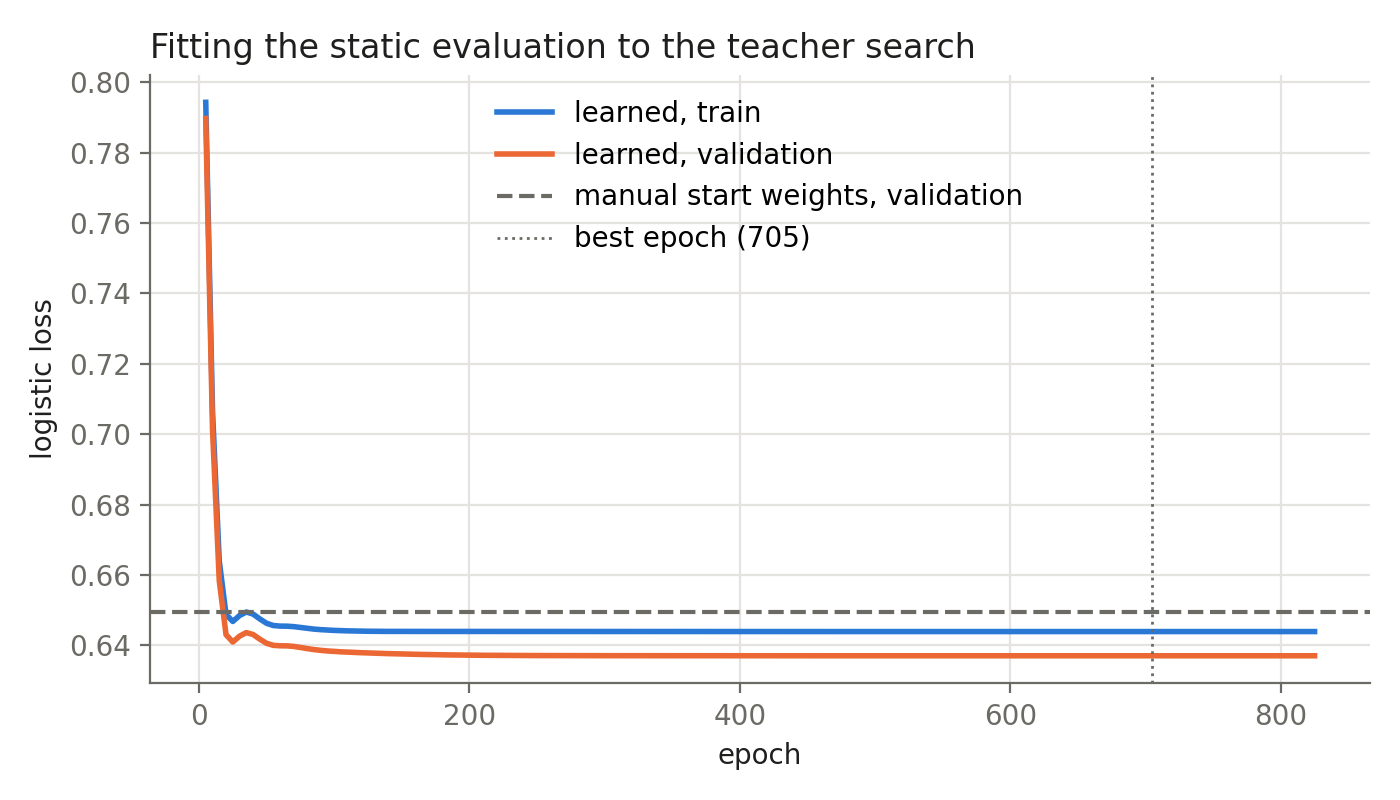
\includegraphics[width=\linewidth]{figures/loss_manual.png}
\caption{ошибка, старт с ручных весов}
\end{subfigure}\hfill
\begin{subfigure}[b]{0.328\textwidth}\centering
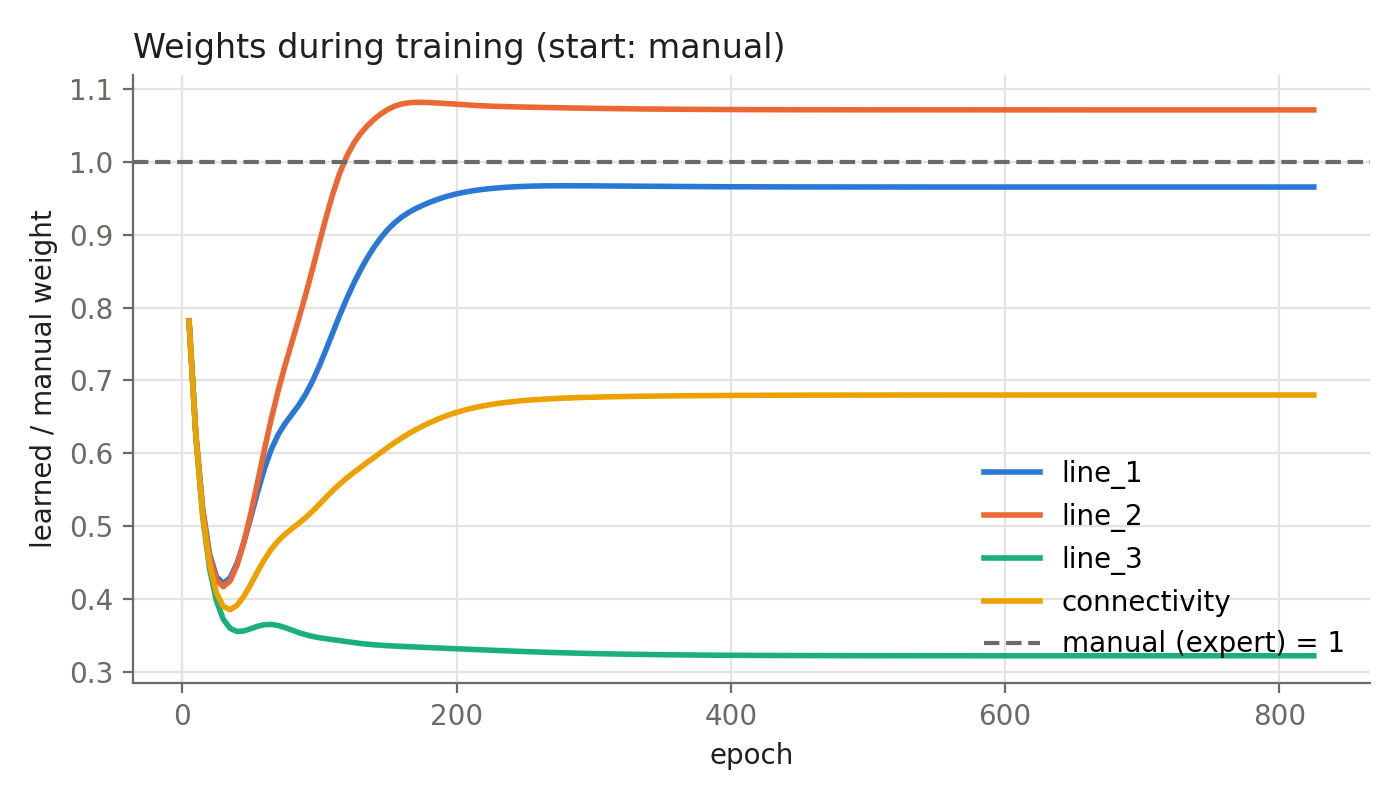
\includegraphics[width=\linewidth]{figures/weights_manual.png}
\caption{веса, старт с ручных}
\end{subfigure}\hfill
\begin{subfigure}[b]{0.328\textwidth}\centering
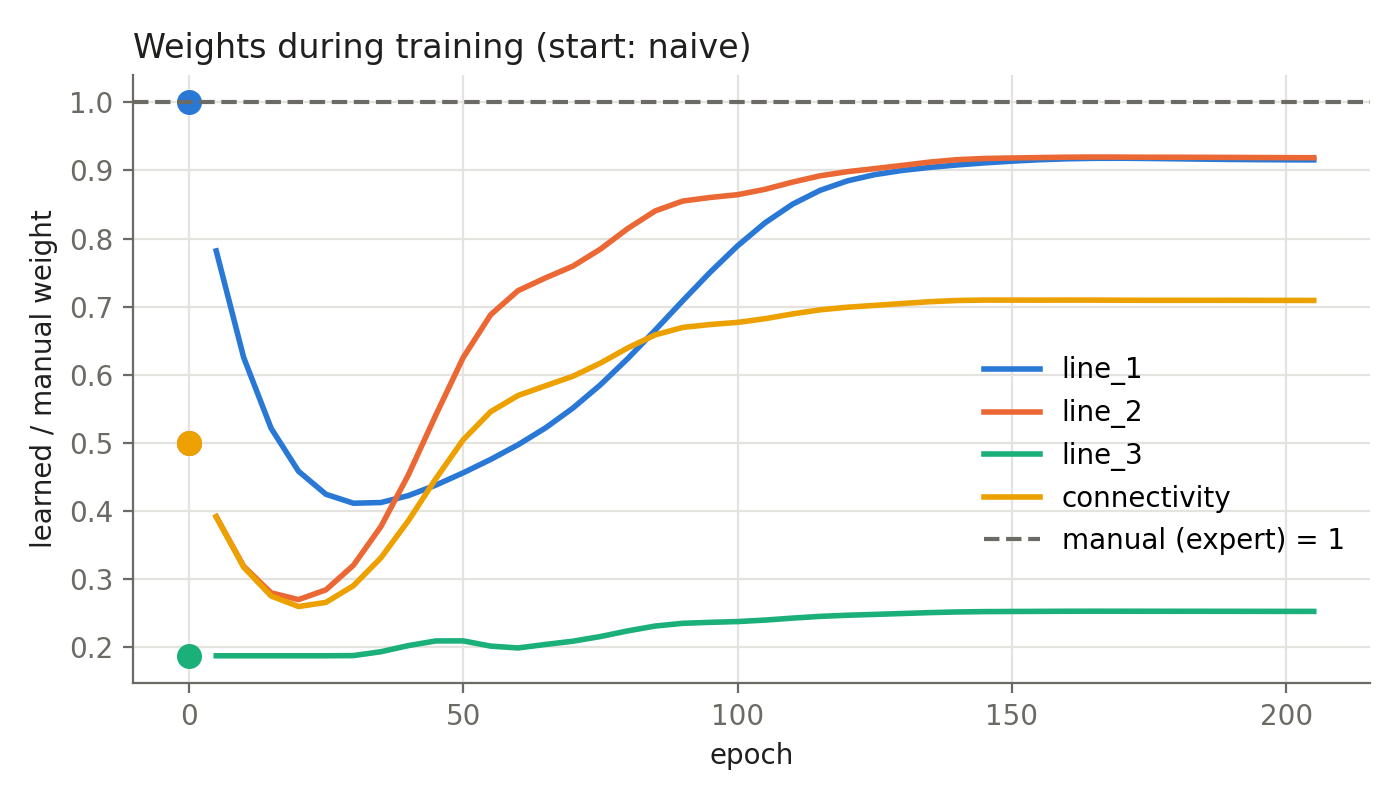
\includegraphics[width=\linewidth]{figures/weights_naive.png}
\caption{веса, старт с наивных (точки)}
\end{subfigure}
\caption{Ход обучения. (a) Логистическая ошибка на train и validation при старте с ручных весов; пунктир --- валидационная ошибка ручных весов (0.6496), лучшая эпоха 705 (0.6371). (b, c) Веса в долях от ручных. Итоговые веса берутся на лучшей эпохе (705 и 85); кривые продолжаются до ранней остановки. Из обоих стартов \code{line\_3} приходит в область 3.7--5.2: сверху (от 16) и снизу (от 3).}
\label{fig:loss}
\end{figure*}

\begin{figure*}[t]
\centering
\begin{subfigure}[b]{0.49\textwidth}\centering
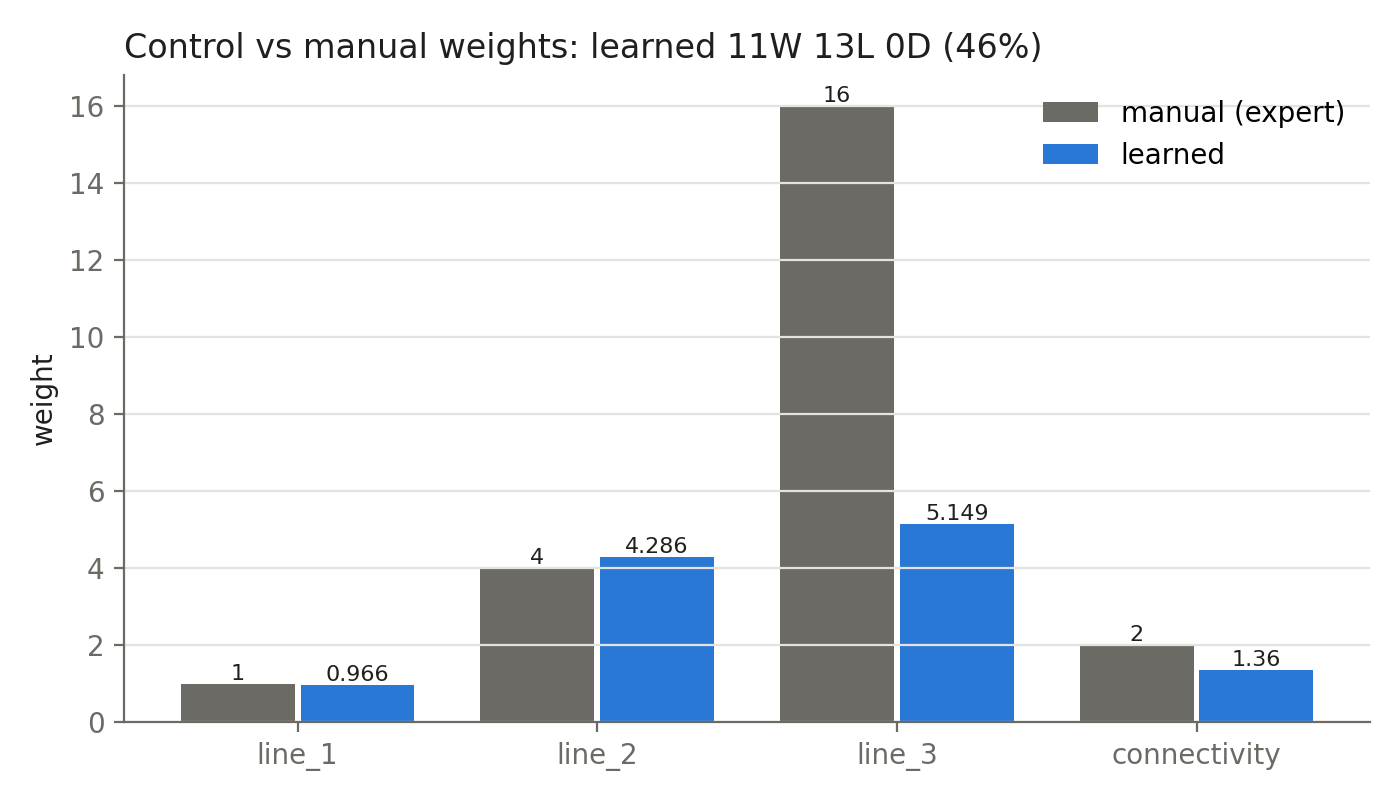
\includegraphics[width=\linewidth]{figures/weights_bar_manual.png}
\caption{ручные и обученные веса}
\end{subfigure}\hfill
\begin{subfigure}[b]{0.49\textwidth}\centering
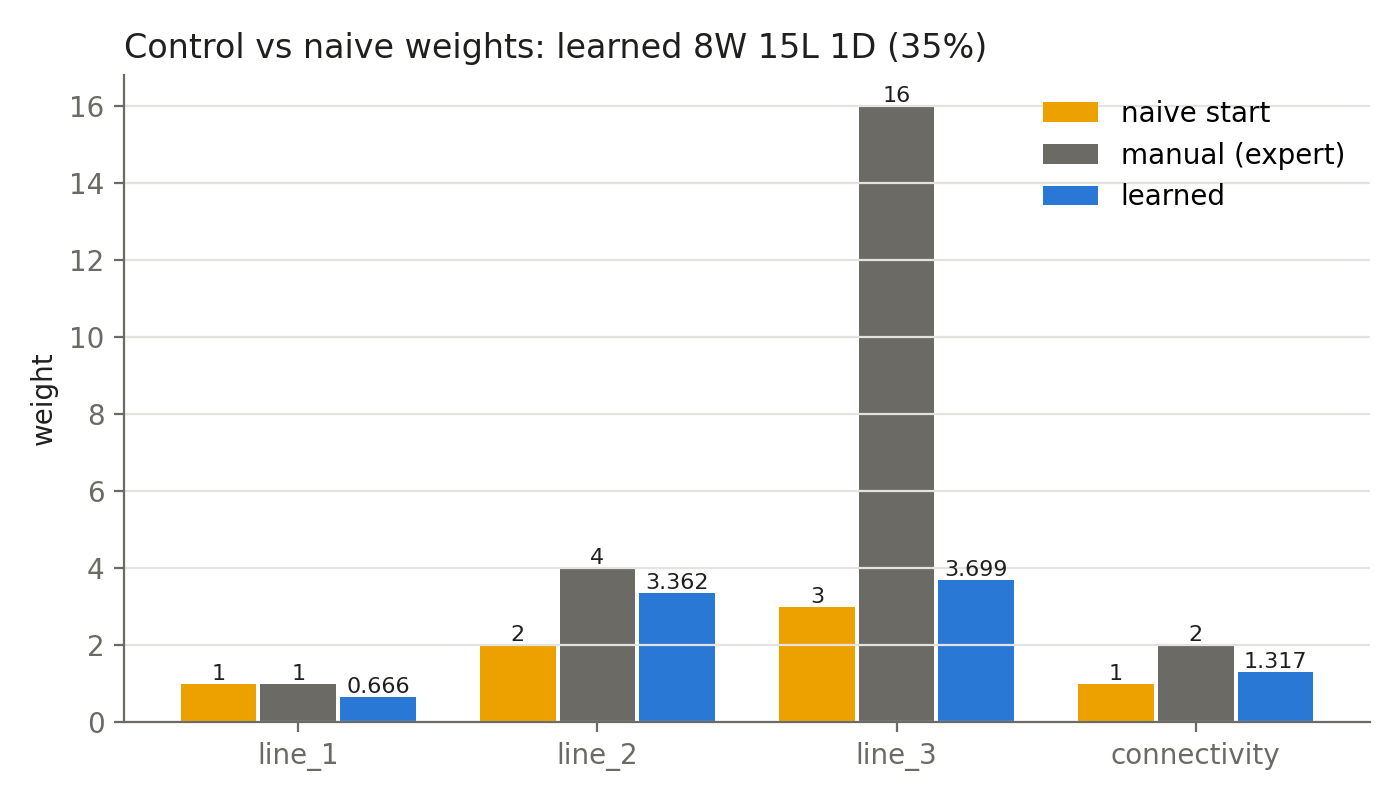
\includegraphics[width=\linewidth]{figures/weights_bar_naive.png}
\caption{наивные, ручные и обученные веса}
\end{subfigure}
\caption{Итоговые веса и результат контрольных партий (в заголовках графиков). Обученные веса из обоих стартов близки друг к другу и далеки от ручного \code{line\_3} = 16.}
\label{fig:weights}
\end{figure*}


\subsection{Weight Learning}\label{sec:learning-results}
Результаты двух запусков обучения --- из ручных и из наивных весов --- приведены в табл.~\ref{tab:learning}, ход обучения и итоговые веса --- на рис.~\ref{fig:loss} и~\ref{fig:weights}.
\begin{points}
\item Процедура работает и из разных стартов приходит в одну и ту же область весов. Из ручных весов \code{line\_3} падает с 16 до 5.1, а из наивных растёт с 3 до 3.7; \code{line\_2} из наивного старта растёт с 2 до 3.4 и почти совпадает с ручным значением 4. Отношение \code{line\_2}/\code{line\_1} в обоих запусках остаётся около 4, что поддерживает выбранное основание 4.
\item При этом функция ошибки почти не различает наборы весов: ручные и наивные веса дают практически одинаковую валидационную ошибку (0.650 и 0.648), а обучение улучшает её лишь на 1--2\,\%.
\item Улучшение ошибки не превращается в силу игры. В контрольных партиях обученные веса набрали меньше 50\,\% в обоих запусках: 45.8\,\% против ручных и 35.4\,\% против наивных весов. Обученные веса занижают \code{line\_3}, а в игре тройки важны: тройка стороны, которая ходит, за один ход превращается в пятёрку.
\item Причина, по-видимому, в устройстве признаков. Каждый признак --- разность «чёрные минус белые», и он не различает, чья тройка: тройка стороны на ходу почти означает выигрыш, тройка соперника --- нет. Линейная модель усредняет эти случаи и занижает \code{line\_3}. Член tempo этого не исправляет: он одинаков для всех позиций и не зависит от признаков.
\item Автоматический выбор в запуске из ручных весов отклонил обученные веса, и это правильное решение: v5 играет ручными весами и совпадает с v4. В наивном запуске выбор оставил стартовые наивные веса; на рабочие веса движка этот запуск не влияет.
\end{points}

\subsection{Tournament}
Все версии и Cloudict сыграли каждый с каждым: 2 дебюта (\code{JJ KJKK} и \code{JJ HHLL}) $\times$ 2 цвета, 3\,с на ход, лимит 30 ходов --- всего 60 партий. 16 партий не закончились за 30 ходов; они засчитаны как ничьи (по 0.5 очка). Итоговая таблица и личные встречи --- в табл.~\ref{tab:tournament}.
\begin{points}
\item Порядок мест совпадает с порядком улучшений: v1, затем v2, v3, v4 = v5 и Cloudict.
\item v3 проиграла v2 личную встречу 1.5:2.5: новая оценка сама по себе силы не добавила, но замедлила поиск в 8 раз. v4 не проиграла ни одной партии ни v2 (2 победы, 2 ничьи), ни v3 (1 победа, 3 ничьи). С учётом раздела~\ref{sec:ablation} разумное объяснение --- ускорение за счёт forward pruning, благодаря которому дорогая оценка v3 укладывается в лимит.
\item Против Cloudict проигрывают все версии, но v2--v5 держатся заметно дольше v1 (в тестах start 11--12.5 своих ходов против 6.5), а v2 и v3 по разу дотянули до лимита 30 ходов. Cloudict сильнее за счёт скорости C++ и поиска VCF на много ходов вперёд, тогда как наш поиск --- два полных хода.
\end{points}

% =====================================================================
\section{Conclusions}\label{sec:concl}

Разработан движок Connect6 \code{tbe}, полностью совместимый с протоколом курса, в пяти версиях; вклад каждого шага измерен.
\begin{points}
\item v1 (минимакс, глубина 2) стала рабочей базой: 614 узлов на ход, проваленные тесты win2, win3 и defend1, 6.5 хода против Cloudict.
\item v2 (alpha-beta, упорядочивание, форсированные ходы) дала самый большой прирост: узлов в 7.7 раза меньше, все 12 тестов пройдены, 11.5 хода против Cloudict.
\item v3 (угрозы по Wu--Huang, связность по Liu) сделала оценку осмысленнее, но в 8 раз дороже; в турнире она уступила v2 со счётом 1.5:2.5.
\item v4 (quiescence, forward pruning) --- лучшая версия: второе место в турнире (11 очков из 20) без поражений от v2 и v3. Отдельный эксперимент показал, что ускорение даёт forward pruning (в 2.7 раза), а quiescence при лимите 3\,с в основном добавляет стоимость.
\item v5 (обучение весов): процедура воспроизводимо сходится из разных стартов, но не улучшает игру (45.8\,\% очков против исходных весов), поэтому автоматический выбор оставил ручные веса.
\end{points}

\emph{Главные уроки.} Генератор ходов и упорядочивание важнее сложной оценки: почти вся тактическая сила появилась уже в v2. Дорогая оценка окупается только тогда, когда поиск успевает её применить, --- в нашем случае благодаря forward pruning. Процедура обучения работает, но её ограничивают признаки: они не учитывают, чья сейчас очередь хода, поэтому функция ошибки почти не отличает хорошие веса от плохих.

\emph{Дальнейшая работа.} (1) Признаки отдельно для стороны на ходу и для соперника --- главное условие, чтобы обучение весов дало эффект. (2) Более глубокий учитель и итеративный бутстрэппинг (переобучение на позициях, сыгранных обученными весами). (3) VCF или поиск в пространстве угроз, как у Cloudict. (4) Таблица транспозиций с учётом симметрий доски и дебютная книга. (5) Турнир v4 только с forward pruning --- возможно, без quiescence движок сильнее.

\bibliographystyle{plainnat}
\bibliography{references}

% =====================================================================
\appendix
\section{How to Run}
\raggedright
Все команды выполняются из папки \code{tbe\_engine}.
\begin{itemize}\itemsep0pt
\item Движок: \code{python3 v5\_final/main.py} (или любая \code{vN\_\ldots/main.py}); в ConnectMore GUI --- \emph{Load Black/White Engine}, затем выбрать \code{v5\_final/main.py}.
\item v4 без оптимизаций: \code{python3 v4\_search\_optimisations/main.py --no-quiescence --no-forward-pruning}.
\item Тесты, метрики и турнир: \code{python3 -B benchmark/benchmark.py}; v4 с выключенными QS и FP: \code{python3 -B benchmark/benchmark.py --ablation}. Нужен собранный Cloudict \code{tbe\_gui/engines/cloudict\_native} (сборка --- \code{cloudict\_native/build.py}).
\item Обучение весов: \code{python3 -B v5\_final/train.py} (старт с ручных весов; итог пишется в \code{learned\_weights.json}) или \code{--init naive}; графики --- \code{python3 -B v5\_final/plot.py}.
\end{itemize}

\end{document}
